\chapter{Travaux réalisés}


\section{Séparation des tâches}
\paragraph{}
Nous constatons assez rapidement dans le projet qu'il est très difficile d'utiliser
le SDK de la Kinect et la DLL directement dans Unity. Plusieurs projets, trouvé durant nos recherche, utilisent un système 
de socket afin de pouvoir envoyer des informations à une application Unity3D à partir d'une application C\#.
Nous utilisons donc la même méthode afin de pouvoir séparer les différentes tâches de notre projet.

\paragraph{}
Nous créons donc un client utilisant la DLL et qui effectue l'ensemble des opérations sur les données afin
de les envoyer à une application Unity3D qui n'a plus qu'à effectuer les transformations sur le modèle avec
les données reçu. En effet, les données fournis pas la DLL ne peuvent être appliqué tel quel sur le modèle.
Le repère des coordonnées fournis par la DLL est le repère image, donc un repère en 2D en pixel. Or, notre 
application doit modèliser la main dans un environnement 3D.

\paragraph{}
Pour avoir une animation de la main la plus précise possible, nous récupérons également les points fournis par
le SDK de la Kinect pour avoir plus d'information, mais également de vérifier les résultats calculés par 
la DLL. Cette vérification ce fait sur le bout du pousse et sur le bout du majeur, car ces points sont communs
à la DLL et au SDK.

\begin{figure}[H]
  \label{carte_main}
  \begin{center}
    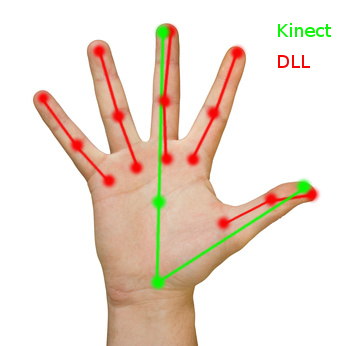
\includegraphics[width=200px]{images/main2.png}
    \caption{Carte des points de la main détectés par la DLL et la Kinect}
  \end{center}
\end{figure}

\paragraph{}
L'intérêt de cette séparation est que notre méthode de localisation des jointures se repose sur une 
DLL et que les calculs effectués sur les données sont spécifiques a celle-ci. En cas de changement de 
technologie, il suffit de modifier le client sans avoir à changer l'application Unity3D. La seul contrainte
étant la structure des socket envoyé. Nous avons donc une application modulable permettant de modifier 
facilement la méthode de récupération les jointures, mais aussi de modifier le matériel utilisé.

\begin{figure}[H]
  \label{schema_application}
  \begin{center}
    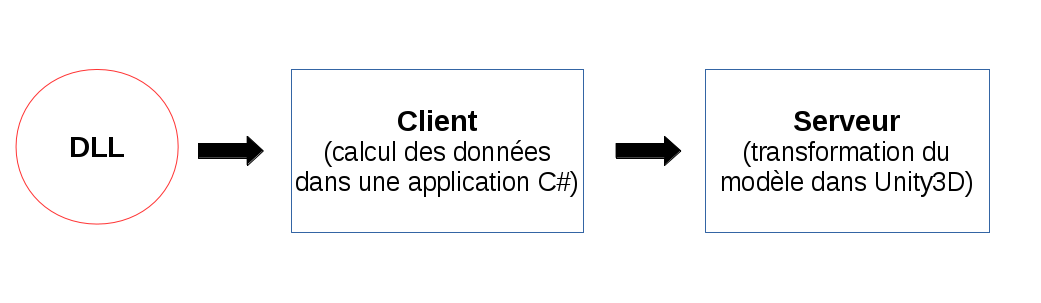
\includegraphics[width=350px]{images/schemaAppli.png}
    \caption{Schéma de la structure de l'application}
  \end{center}
\end{figure}

\section{Récupération de la position des jointure de la main}
\paragraph{}
Le premier problème à résoudre est donc le calcul de la troisième coordonnée de chaque jointure. Grâce à la Kinect,
il est possible de récupérer les coordonnées, dans le repère monde, de la jointure du poignet. Elle nous permet
également de récupérer une valeur dans l'image de profondeur, valeur représentant la troisième coordonné d'un point.
Nous avons alors la valeur du pixel de l'image de profondeur de la jointure recherché $p_{recherche}$, la valeur
du pixel de l'image de profondeur de la jointure du poignet $p_{ref}$ et la valeur de la troisième coordonné dans 
le repère monde de la jointure du poignet $z_{ref}$. Nous appliquons alors une règle de trois pour obtenir 
la valeur dans le repère monde de la troisième coordonné de la jointure courante.

\begin{equation}
 z_{recherche} = \frac{z_{ref} * p_{recherche}}{p_{ref}}
\end{equation}

\paragraph{}
La seconde problématique de notre méthode est la normalisation des coordonnées que nous avons récupérer. Les coordonnées
de la kinect sont dans le repère monde, nous avons donc besoin d'utiliser les caractéristiques de la caméra pour normaliser
les coordonnées. Nous prenons une distance de 4m pour la profondeur maximum de la caméra, car cela correspond à la profondeur 
de champ de la Kinect.

\paragraph{}
Enfin la dernière problématique est la rotation de la main. Jusqu'à maintenant, nous ne fessons qu'appliquer les coordonnées
fournies dans les sockets, mais il n'y a aucune rotation appliqué sur la main. Lorsque la main est bien parallèle à la caméra,
le poignet reste perpendiculaire à celle-ci et les doigts sont parallèles. Pour palier à cette problématique nous avons calculé
l'angle entre la droite représentant l'horizontal et la droite passant le poignet et le bout du majeur.
%TODO prendre un screenshot de l ecran pour le problème de rotation de la main

%TODO prendre une image de la main avec un axe horizontal et l'angle à calculer

\section{Modélisation et animation de la main}
\paragraph{}
Nous avons choisi de ne pas modéliser la main de l'utilisateur, à la place, nous avons récupérez un modèle de main existant sur Internet.
Sous Blender, nous y avons appliqué une armature pour pouvoir l'animer de façon réaliste. Cette armature est constituée d'os et de jointures. On peut considérer que l'armature est un arbre avec les noeuds qui sont des os et les arcs qui sont les jointures. Les transformations de chaque fils dépend des transformations de leurs père. Ainsi, un mouvement du poignet entraine le mouvement de chaque os de la main. 
Cette armature pourra être utilisée pour mimer la main de l'utilisateur. 

\paragraph{}
Pour relier l'armature au modèle, on utilise une méthode de skinning. Le skinning est expliquée dans l'état de l'art. Dans Blender, on peut utiliser différent types de skinning, soit \og à la main \fg en créant des groupes de sommets à associer à chaque jointures, soit en utilisant des algorithmes de création des groupes et d'attribution automatique des sommets à ces groupes. Nous avons choisi d'utiliser la méthode \og bone heat \fg. \cite{baran2007automatic}

\paragraph{}
Le modèle et armature ainsi créés sont importés dans Unity3D tout en conservant les associations effectuées par le skinning. Ensuite, on teste ce modèle en l'animant à l'aide de rotations des jointures, on peut ainsi faire prendre des poses à la main. 

\begin{figure}[!h]
	\centering
	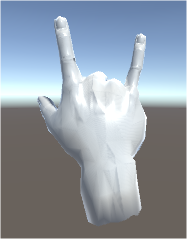
\includegraphics[width=0.45\textwidth]{images/HandPose1.png}
	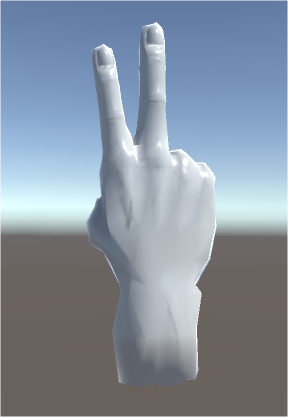
\includegraphics[width=0.46\textwidth]{images/HandPose2.png}
	\caption{Poses réalisées à partir de rotations des jointures de l'armature dans Unity}
\end{figure}

\paragraph{}
Les différentes techniques d'animation basé sur une armature sont décrites dans l'état de l'art correspondant. 
Pour notre projet, nous avons choisi la méthode qui utilise les articulations récupérées par la DLL en conjonction avec les points récupérés \textit{via} le SDK de la Kinect. 
Ces points servent à positionner les jointures de l'armature par translations et/ou rotations.\newline
On utilise les points suivants détectés par la Kinect : le poignet, le milieu de la main et le sommet du pouce pour positionner et orienter le modèle en concordance avec les points détectés par la DLL.
Pour cela, on applique une translation du modèle, vers la position du poignet détecté. Puis on calcule l'angle entre les vecteurs $V_{AB}$ et $V_{CB}$  : 

\begin{figure}[H]
\centering
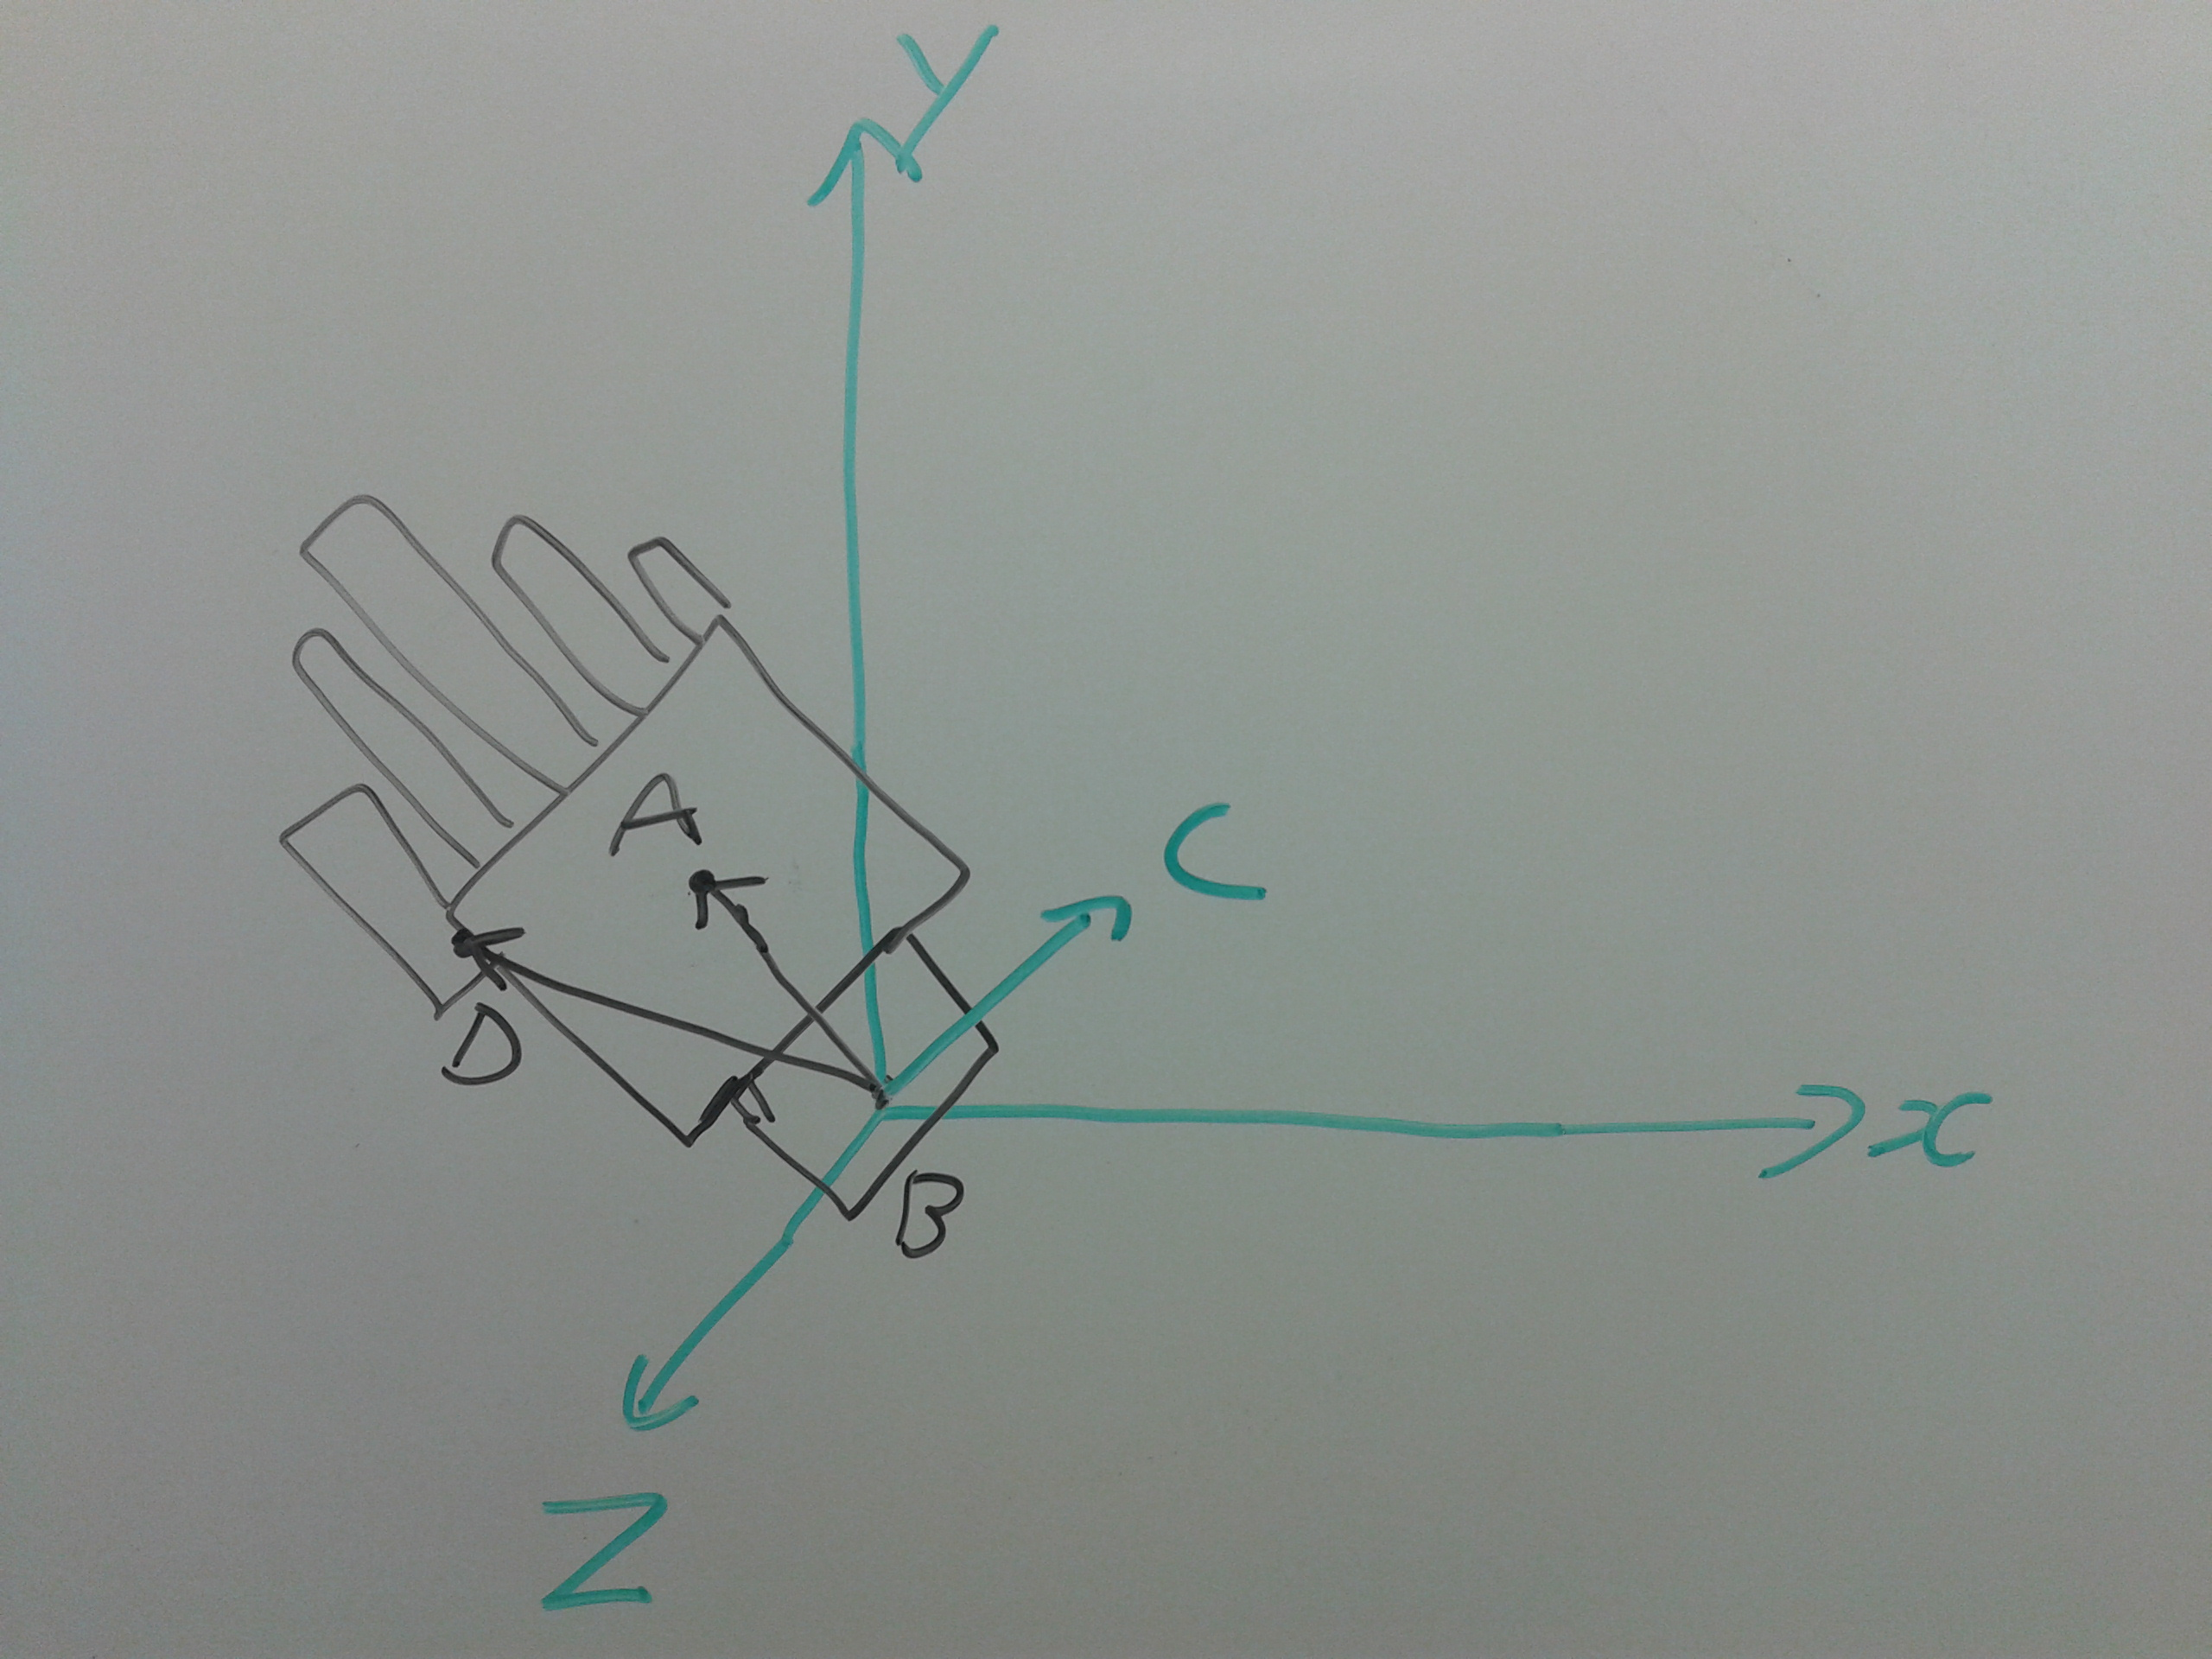
\includegraphics[width=0.7\textwidth]{images/SchemaRotationMain.jpg}
\caption{Schéma d'explication du calcul des vecteurs utilisés pour calculer la rotation du poignet}
\end{figure}

On applique une rotation de l'angle calculé à l'armature du modèle, cela permet de retrouver l'orientation de la main sur l'axe X et Y.
Une opération similaire est effectuée avec la base du pouce à la place du milieu de la main pour trouver l'orientation en Z: 


\paragraph{}

Une fois le modèle correctement positionné et orienté, il faut s'occuper des doigts. Une partie complexe a été de décider d'une méthode de calcul des angles des jointures et de l'implémenter.
Nous avons choisi de calculer les angles de la même façon que pour le poignet (à l'aide de vecteurs) et sur le même principe.\\
Les vecteurs sont formés par les points suivants : la jointure qui sert de pivot et le point suivant dans l'armature forment un vecteur, ainsi que la jointure (pivot) et le point détecté par la DLL correspondant au point de l'armature. (cf. Figure 3.5)

\newpage

\begin{figure}[H]
 \centering
 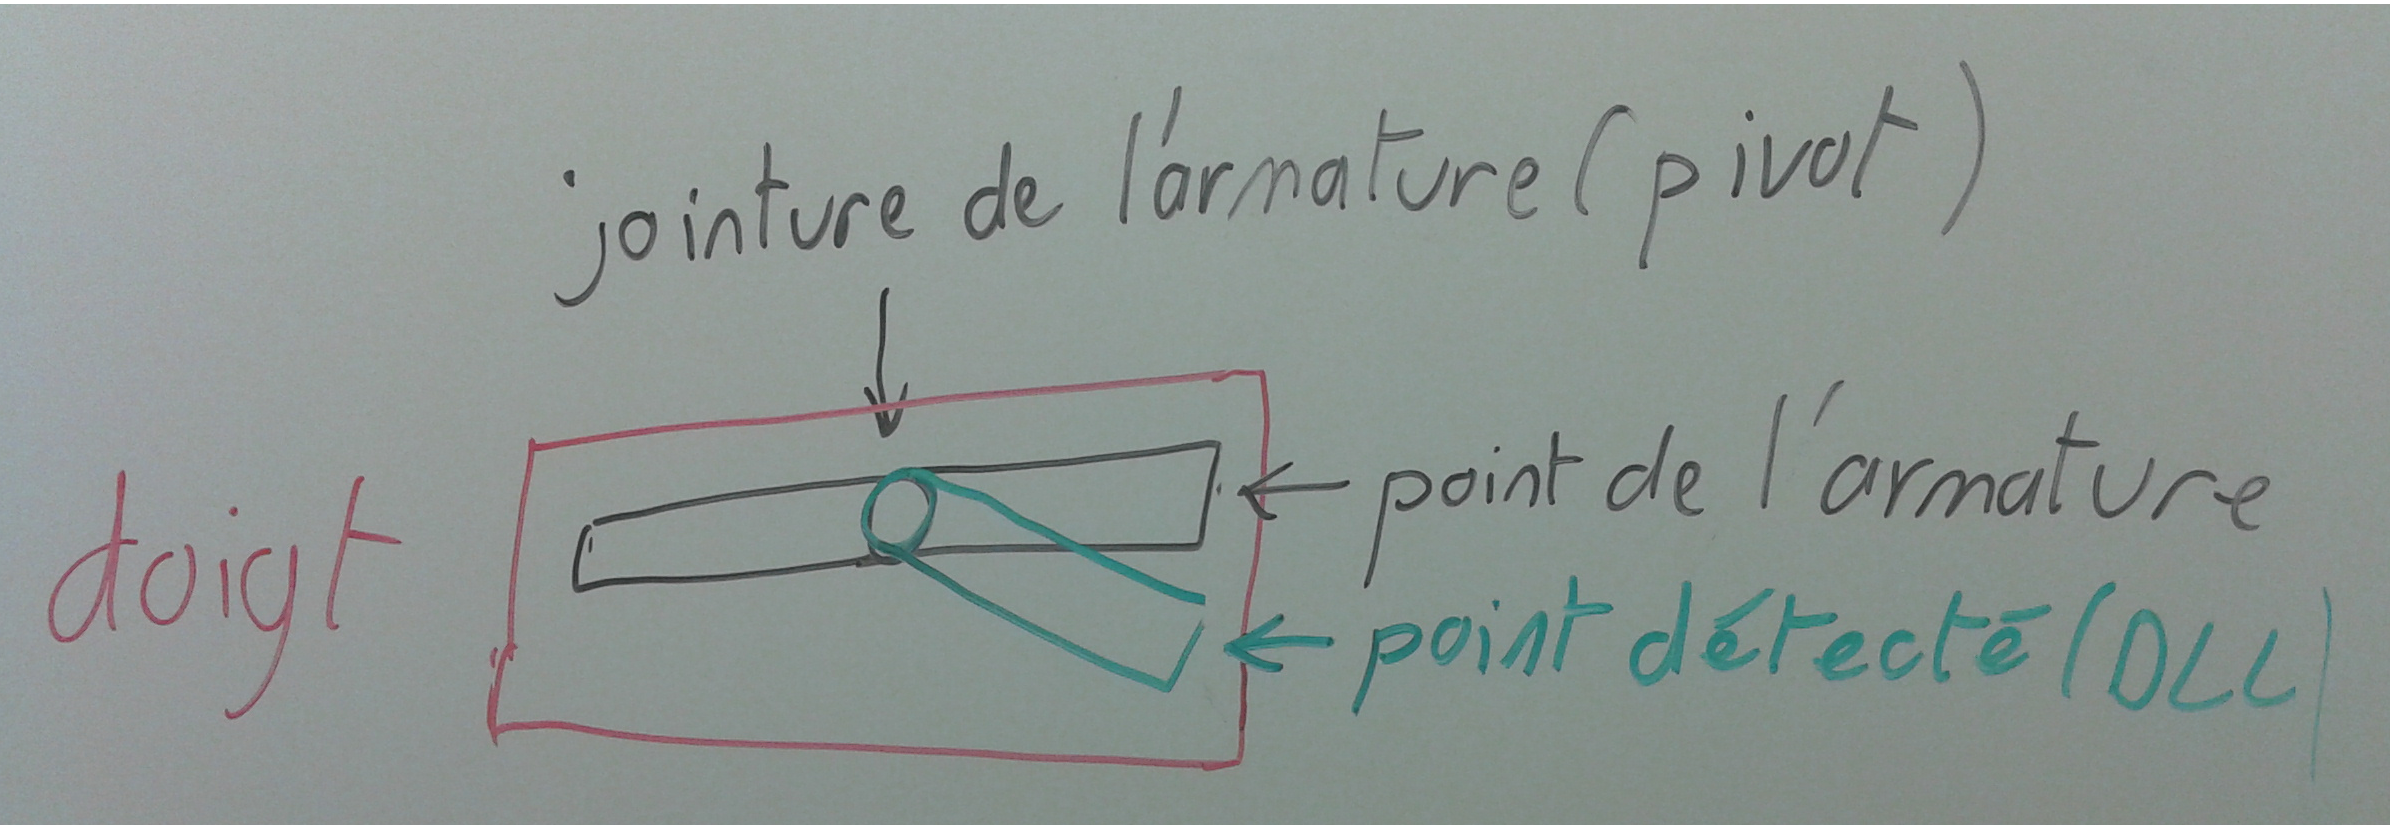
\includegraphics[width=0.7\textwidth]{images/SchemaRotationDoigt.png}
 \caption{Schéma d'explication du calcul de l'angle aux jointures de l'armature}
\end{figure}

\section{L'application de démonstration}